\chapter{Developmental stability of the \abbr{mrna}--\abbr{trna} interface}
\label{sec:trna}

To study how changes in \mrna gene expression relate to changes in \trna gene
expression, we collected tissue samples from six time points in mouse (\mmu)
development: two before birth (E15.5 and E18.5, which stands for \num{15.5} and
\num{18.5} days after gestation of the oocyte, respectively); two shortly after
birth, happening around E20 (P0.5 and P4 --- \num{0.5} and \num{4} days after
birth, respectively) and two after weaning the juvenile mice (P22 and P29).

For each of these time points, tissue was collected from whole liver and whole
brain (\define[\defineword{homogenise} breaking apart and mixing the tissue in
such a way that all the cell types will be evenly distributed throughout the
sample]{homogenised}) and prepared for \rnaseq and \pol3 \chipseq in order to
assay \mrna and \trna gene expression. The tissues were chosen for their
interesting shifts in physiology during development: the liver is a homogeneous
organ predominantly made up of a single cell type --- around \num{70} per cent
hepatocytes --- and liver function changes fundamentally at birth; prenatal
liver serves mainly as a haematopoietic organ, whereas liver of post-natal mice
is primarily a metabolic organ \citep{Si-Tayeb:2010}. Brain, by contrast, is a
highly heterogeneous organ made up of many different cell types, with dynamic
changes all through development \citep{Liscovitch:2013}.

\Cref{fig:trna-project-outline} summarises the experimental
procedure.\footnote{The wet-lab work of this project was performed by Bianca
Schmitt, who was also a joint first author on the manuscript. Claudia Kutter
provided guidance with the interpretation of the results and helped with the
creation of the figures.} Each experiment was performed in two biological
replicates, which were highly correlated
(\cref{fig:trna-replicate-variability}). \Cref{tab:variables} summarises the
variable names used to refer to data throughout this chapter.

\textfig[\todo{Remove background gradients from graphics}]
    {trna-project-outline}{body}{0.8\textwidth}
    {Sample analysis outline.}
    {Samples were collected in eight distinct time points. Of these, E9.5 and
    E12.5 were excluded from most of the subsequent analysis, except where
    noted. For each time point, tissue was collected from liver and brain, and
    on the one hand prepared for \rnaseq, and on the other hand cross-linked to
    the \pol3 antibody and prepared for \chipseq. The resulting data was used to
    quantify \mrna and \trna gene expression, codon usage and \trna anticodon
    abundance. Figure created by Claudia Kutter.}

\textfig{trna-replicate-variability}{body}{0.5\textwidth}
    {Replicate variability.}
    {Shown are the Spearman correlation coefficients between pairwise biological
    replicates for the \trna count data (left) and the \mrna count data (right).}

\begin{table}[!ht]
    \centering
    \begin{tabular}{@{}lll@{}}
        \toprule
        & \abbr{mrna} & \abbr{trna} \\
        \midrule
        Raw counts per replicate & \(m_{ij}\) & \(t_{ij}\) \\
        Normalised counts per replicate & \(m_{ij}^*\) & \(t_{ij}^*\) \\
        Counts of merged replicates & \(m_{iy}'\) & \(t_{iy}'\) \\
        (Anti-)codon level counts & \(c_{xy}\) & \(a_{xy}\) \\
        \bottomrule
    \end{tabular}
    \tabcap{variables}
        {Summary of the matrix and subscript names.}
        {\(i\) is the index of a gene; \(j\) is the index of a library
        replicate; \(x\) is an (anti-)codon;  \(y\) is the index of a
        developmental stage.}
\end{table}

In addition to the six time points described above, tissue was also collected at
two earlier stages, E9.5 and E12.5. However, the embryo at such early stages of
development is too small, and the tissue development has not progressed far
enough, to permit collecting enough tissue-specific material. For that reason we
used the whole embryo at E9.5 and separated the E12.5 embryo into torso and
upper body. The subsequent analysis was performed on the six later stages in
liver and brain. However, the earlier stages confirmed the general patterns
found by analysing the remaining data (\cref{fig:pca-all-stages}).

The analysis and the results presented in this chapter are published as
\texttitle{High-resolution mapping of transcriptional dynamics across tissue
development reveals a stable \mrna[–]\trna interface} [Schmitt,
Rudolph,\andothersdelim\& al., \cite*{Schmitt:2014}].

\section{Protein-coding gene expression changes dynamically during mouse
development}

To investigate protein-coding gene expression changes during development, we
quantified the \mrna abundance from \rrna-depleted \rnaseq data (strand-specific
\SI{75}{bp} paired-end reads from \name{Illumina} \name{HiSeq~2000}). Reads were
mapped to the \mmu reference genome (\abbr{ncbim37}) using
\name{\lowsc{i}\abbrsc{RAP}} \citep{Fonseca:2014} and \name{TopHat2}
\citep{Kim:2013}. Read counts were quantified using \name{HTSeq}
\citep{Anders:2014}, and assigned to protein-coding genes from the
\name{Ensembl} release \num{67} \citep{Flicek:2014}.

We excluded mitochondrial chromosomes from the analysis, because mitochondrial
genes use a slightly distinct genetic code \citep{Osawa:1989}. Furthermore, we
excluded sex chromosomes.

Changes in the expression of protein-coding genes, leading to changes in
abundance of proteins, are known to drive cellular behaviour
\citep{Brawand:2011}. Our data confirms that tissue development in mice is
accompanied by large-scale changes in the \mrna transcriptome. This is nicely
illustrated by looking at individual gene expression counts, plotted against
their genomic location (\cref{fig:mrna-expression-change}). For example, in the
liver we can confirm the functional relevance of apolipoprotein B
(\protein{APOB}) as the primary carrier of lipoproteins, which becomes
increasingly relevant as the organ shifts to metabolism \citep{Knott:1986}.
Similarly, \mrna gene expression changes highlight the role of α-fetoproteine
(\protein{AFP}) as the fetal version of serum albumin (\cref{fig:apob-afp})
\citep{Chen:1997}. In the brain, shifts can be seen in the activity of the
neural \tf \protein{FOXP2}, the expression of which continuously decreases, and
in calmodulin (\protein{CALM1}), where transcription increases after birth
\citep{Tsui:2013,Huang:2011}.

\textfloat{mrna-expression-change}{spill}{%
    \centering
    \begingroup
        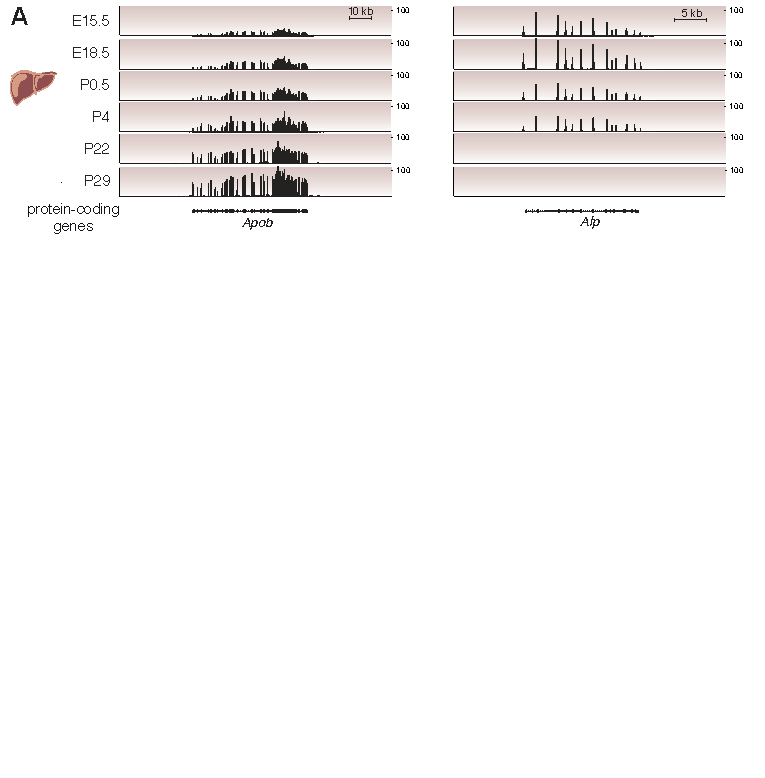
\includegraphics[width=\textwidth]{liver-mrna-expression-change}
        \vspace{-\baselineskip}
        \subcaption{\label{fig:apob-afp}Gene expression changes of
            \gene{mmu}{Apob} and \gene{mmu}{Afp}.}
        \vspace{\baselineskip}
    \endgroup
    \par
    \begingroup
        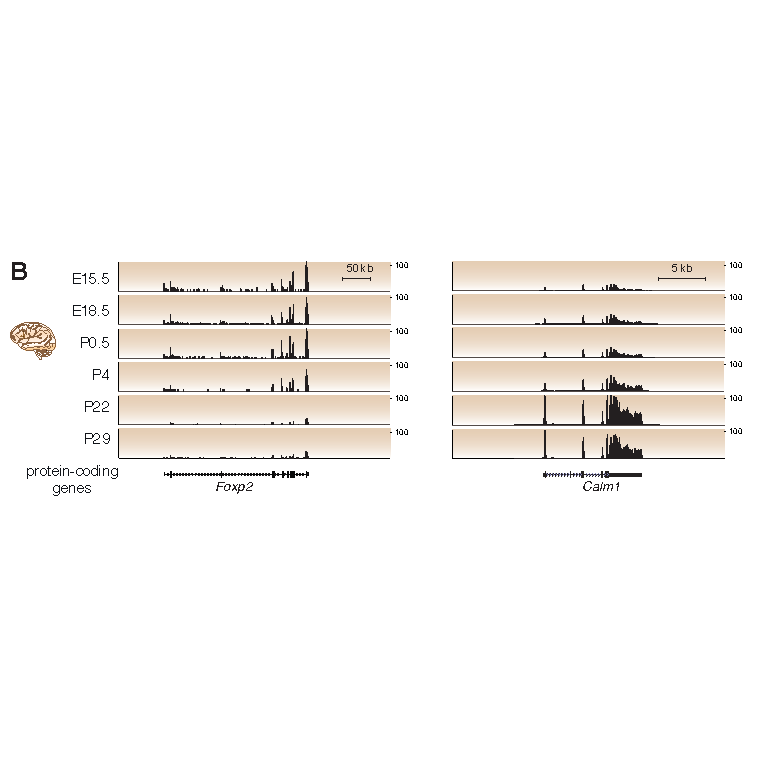
\includegraphics[width=\textwidth]{brain-mrna-expression-change}
        \vspace{-\baselineskip}
        \subcaption{Gene expression changes of \gene{mmu}{Foxp2} and
            \gene{mmu}{Calm1}.}
    \endgroup}
    {Example of gene expression changes in development.}
    {The four genes are representative for tissue- and stage-specific genes,
    whose expression changes drive cell function. These changes can go up or
    down over the course of development, correspoding to either an up- or
    downregulation. Figure created by Bianca Schmitt.}

For a more systematic analysis, I took the matrix of normalised count data of
all library replicates and all \mrna[s], \(m_{ij}^*\), for each \mrna gene \(i\)
and each library replicate \(j\), and calculated the pairwise Spearman rank
correlation between all replicates,

\begin{equation}
    cor_{ij} = \operatorname{cor}(m_{\cdot i}^*, m_{\cdot j}^*) \text{\ for all
        libraries \(i\), \(j\),}
\end{equation}

where \(m_{\cdot i}^*\) denotes the \(i\)th column of the matrix \(M^*\).

I then performed \pca on the correlation matrix, which allows variation in the
data to be projected onto uncorrelated axes, so that the first axis represents
the component that explains the most variance of the data, and the second axis
represents the second component.

The resulting \pca in \cref{fig:mrna-pca} shows that the biggest source of
variance in the correlation structure of the expression data is tissue identity,
which explains \num{97} per cent of the total variance. However, of the
remaining variance, \num{60} per cent is explained by progression of tissue
development in a way that nicely mirrors the known biology: the plot’s \(y\)
axis shows the linear progression of development from early stages at the bottom
to late stages at the top. We observe a much stronger variation on the \(y\)
axis for liver data: this could be explained by noting that the liver is more
homogeneous than the brain, and changes in gene expression are therefore more
coordinated; it might also reflect the change in liver function from a
haematopoietic to a metabolic organ around birth.

Next, I used \name{DESeq2} \citep{Love:2014} to identify differentially
expressed genes between stages and tissues. Genes are counted as differentially
expressed if their Benjamini–Hochberg \fdr-corrected \(p\)-value is below
\num{0.001}. The number of differentially expressed genes between all pairwise
developmental stages unsurprisingly shows that more distinct developmental
stages have higher numbers of differentially expressed genes
(\cref{fig:mrna-de-matrix}). Furthermore, there is a clear gap between pre- and
post-weaning stages, with a large jump in the number of differentially expressed
genes across the weaning boundary, in both liver and brain.

\textfigtwo{mrna-pca}
    {\pca of \mrna gene expression per developmental stage.}
    {Rotations \num{1} and \num{2} of the correlation matrix of
    protein-coding gene expression in each developmental stage. The percentage
    on the axes shows the amount of variance explained by each rotation.}
    {mrna-de-matrix}
    {Number of differentially expressed \mrna genes between stages:}
    {Each off-diagonal square shows the number of differentially
    expressed genes (at a significance threshold of \(p<0.01\)) between
    the two indicated developmental stages.}

These patterns are noteworthy because they recapitulate tissue identity and
linear progression through the stages of tissue development. But they are not
particularly surprising: cell function is dictated by the abundance of specific
proteins and thus protein-coding gene transcription. The patterns of gene
expression similarity shown in the \pca and in the number of differentially
expressed genes hence recapitulate the expected changes in cell function between
tissues and through development.

\section{Dynamic changes of \abbr{trna} gene expression during mouse
development}

Quantification of \trna genes was performed by first mapping the \pol3 \chipseq
data (non-strand-specific \SI{36}{bp} single-end reads sequenced by
\name{Illumina} \name{Genome Analyzer~IIx} or \name{HiSeq~2000}) using
\name{\abbrsc{BWA}} version 0.5.9-r16 \citep{Li:2009a} using default parameters.
Next, non-uniquely mapping reads were reallocated probabilistically according to
the description given in the previous chapter, using the \trna gene annotation
from the \name{Genomic \trna Database}, described in \citet{Chan:2009}. For each
\trna gene (again excluding mitochondrial \trna genes because the genetic code
of the mitochondrial \mrna genes differs from the nuclear genetic code), reads
were summed within each \trna gene locus and in the \SI{\pm100}{bp} flanking
regions.

\trna genes that were unexpressed in all experimental conditions were excluded
from further analysis, to reduce the effect of multiple testing
\citep{Bourgon:2010} and to exclude potential pseudogenes in the annotation. To
be called expressed, a \trna gene had to be present in all replicates of at
least one condition with a count of at least \num{10}, after size-factor
normalisation. The threshold \num{10} was chosen so that small variations in
either direction would have a minimal impact on the thresholding. The following
analysis is thus performed using \num{311} expressed out of \num{433} total
\trna genes (\num{72} per cent).

Unlike proteins, \trna[s] do not perform a cell type specific function; instead,
their continued presence is required for the maintenance of transcription in all
cellular conditions. We therefore did not expect many changes in the levels of
\trna gene expression over the course of development, and we do in fact observe
that many \trna gene expression levels remain stable (\cref{fig:trna-counts}).
Nevertheless, we also observe that around \num{50} per cent of all \trna genes
\emph{are} differentially expressed. \Cref{fig:liver-trna-expression-change}
shows a genomic locus containing \trna genes that displays these different
dynamics.

\textfigtwo{trna-counts}
    {Overview over \trna gene expression change.}
    {Bar plots show different types of \trna gene expression dynamics: \trna
    genes without change in their expression levels, \trna genes with changes to
    their expression levels, which are nevertheless expressed in all stages of
    development across both tissues; and \trna genes which are only expressed in
    a subset of all conditions. Figure created by Claudia Kutter.}
    {liver-trna-expression-change}
    {Example of dynamically changing \trna genes.}
    {Genomic region showing different types of \trna gene expression behaviour;
    the label colours on the x axis corresponds to the colours in
    \cref{fig:trna-counts}. Figure created by Bianca Schmitt.}

Surprisingly, the \trna gene expression differences follow similar patterns to
those observed in \mrna genes, with the first two principal components resulting
from the application of \pca to the rank correlation matrix again corresponding
to the tissue an developmental stage (\cref{fig:trna-pca}). The observed
patterns are incompatible with mere \emph{random} expression changes (which
would result in an unordered cloud of points). Something must account for these
concerted changes in \trna gene expression.

\textfig{trna-pca}{body}{0.8\textwidth}
    {\pca of \trna gene expression per developmental stage.}
    {Rotations \num{1} and \num{2} of the correlation matrix of
    \trna gene expression in each developmental stage. The percentage on the
    axes shows the amount of variance explained by each rotation.}

In the case of the protein-coding genes, we can explain the nonrandom changes in
gene expression by known gene regulatory mechanisms, which control the
transcriptome of each cell and developmental stage. The fact that \trna gene
expression changes across development exhibit the same patterns as \mrna gene
expression changes suggests that \trna gene expression is subject to similar
regulatory constraints. We therefore attempted to explain \emph{why} \trna gene
expression requires changing in a regulated manner, and \emph{how} this \trna
gene regulation is carried out by the cell.

Our first suspicion was that changes in \mrna gene expression might lead to
changes in codon demand, since different protein-coding genes are made up from
different codons. The change in codon demand in turn could lead to a change in
anticodon supply in the form of differential \trna gene expression. This would
meet the need for efficient translation: mismatching codon and anticodon pools
would either lead to a wasteful over-production of \trna[s] of a given
anticodon, or to a bottleneck in such an anticodon supply, causing efficiency
loss in translation. Both scenarios present a suboptimal scenario for the
fitness of the cell and should reasonably be selected against. In fact, there is
some evidence that such a selection takes place
\citep{Ikemura:1981,Ikemura:1985,Yang:2008}.

We therefore went on to quantify the codon pool corresponding to each given
transcriptome, as well as the pool of available \trna genes, grouped by their
anticodon isoacceptor identity.

\section{Every mouse \abbr{mrna} transcriptome encodes the same distribution of
triplet codons and amino acids}

The codon pool of a given \mrna transcript is given by the distribution of
triplet codons in its sequence. There are \num{64} possible triplet codons, of
which \num{61} encode \num{20} different amino acids, and three encode the stop
codon, marking the end of translation.\footnote{The analysis ignores
selenocysteine, which is a \num{21}st possible amino acid, and which can be
encoded by the stop codons \codon{UGA} under rare circumstances (see
\cref{sec:trna-intro}).} Using this information and the transcript abundance
quantified by our \rnaseq data, I calculated the abundance of each triplet codon
as well as each amino acid in the transcriptome of each developmental stage. I
then compared these across stages to find out how they varied.

First, for every gene, the number of occurrences of each codon in the longest
annotated transcript (which is often called the “canonical”
transcript\footnote{\url{http://www.ensembl.org/Help/Glossary?id=346}, retrieved
2014-05-12.}) was determined and this value was multiplied by the gene’s
expression (normalised for transcript length):

\begin{equation}
    c_{xiy} = \text{codon}_{xi} \cdot \frac{m_{iy}'}{l_{i}} \text{\ ,}
\end{equation}

where \(\text{codon}_{xi}\) is the number of occurrences of codon \(x\) in the
canonical transcript of gene \(i\), \(m_{iy}'\) is the gene expression count of
gene \(i\) in condition \(y\) (averaged across the replicates of condition \(y\)
after library size normalisation), and \(l_i\) is the length of the canonical
transcript of gene \(i\).

Next, the overall usage of each codon was obtained by summing these values
across all genes:

\begin{equation}
    c_{xy} = \sum_i c_{xiy} \text{\ .}
\end{equation}

Relative codon usage (\rcu) values \(c_{xy}^*\) were then calculated by dividing
each codon usage value by the sum of the codon usage values of a given
condition:

\begin{equation}
    c_{xy}^* = \frac{c_{xy}}{\sum_{k\in \operatorname{syn}(x)} c_{ky}} \text{\ ,}
\end{equation}

where \(\operatorname{syn}(c)\) is the set of synonymous codons to which \(c\)
belongs.

We find that at the transcriptome level, codon abundance is highly stable across
development in both tissues (Spearman’s \(\rho > 0.97\)) ---
\cref{fig:codon-anticodon-abundance} top left shows this by way of example using
the codons for arginine in the different stages in liver.

Given this stability, I next explored how much variation should be expected for
varying transcriptomes, by simulating random transcriptomes and computing their
codon usage.

I used our library-size normalised \rnaseq data to simulate background
distributions in liver and brain for each specific developmental stage. I
randomly rearranged the expression values across genes for the expressed
(“\textsc{expr}”) and all genomically annotated (“\textsc{all}”) protein-coding
genes. For each developmental stage, I created \num{100} such random background
distributions. I then calculated the triplet codon usage for the rearranged
protein-coding \rna expression distributions.

\Cref{fig:codon-anticodon-abundance} top middle and right shows that, even for
simulated transcriptomes, the codon usage remains unchanged. In fact, both
observed and simulated transcriptomes seem to simply reflect the codon abundance
found in the coding part of the genome, regardless of the sometimes strong
variations in gene expression between different transcriptomes.

\begingroup% Necessary to prevent paragraph indent vanishing subsequently.
\textfloatbare{spill}
    {\ifoddpage\else\raggedleft\fi%
    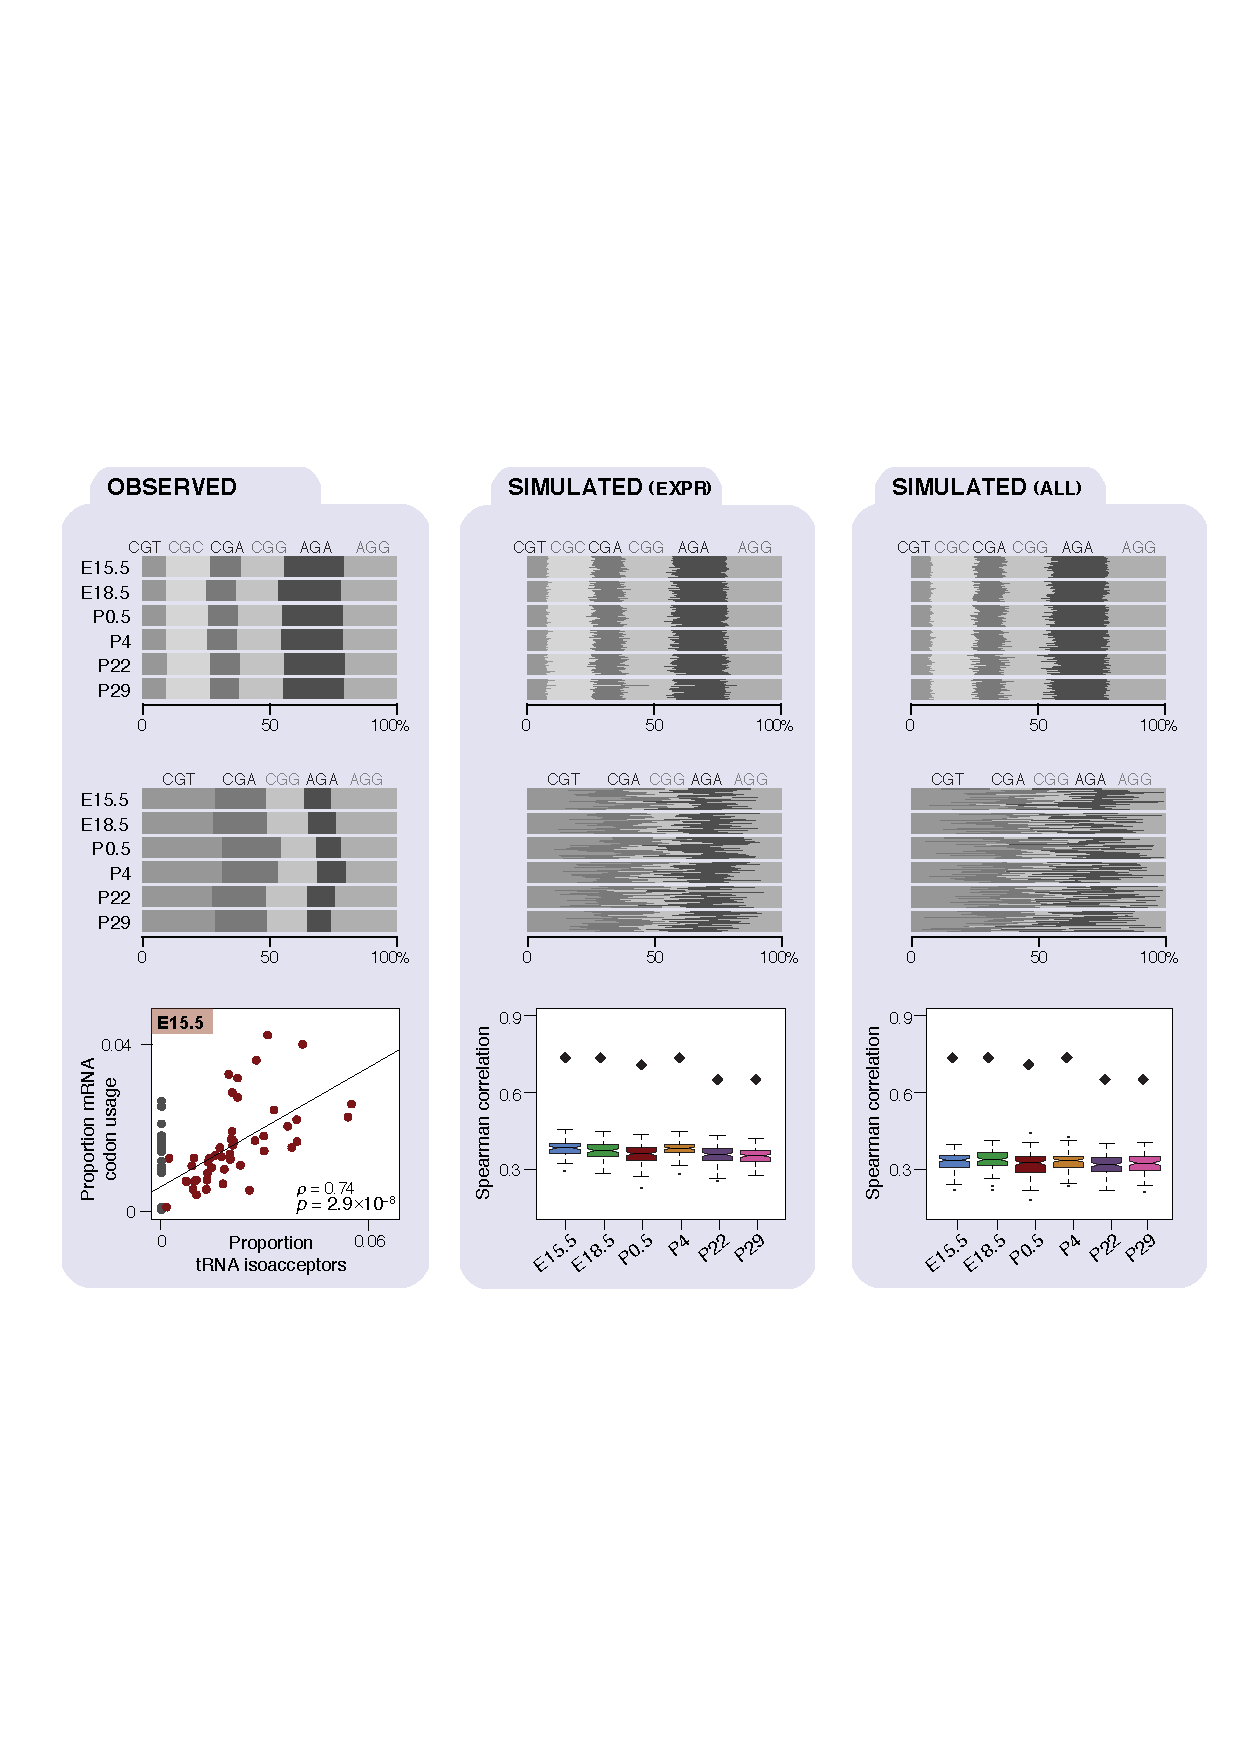
\includegraphics[width=0.95\textwidth]{codon-anticodon-abundance}}{}

\vspace{-\baselineskip}
\figcapof{codon-anticodon-abundance}
    {Codon and anticodon abundance across stages of development.}
    {The figure consists of three panels (right, middle, left) with three
    subfigures (top, centre, bottom) each. The left panel shows observed data
    for each of the developmental stages in liver (brain data is comparable).
    The middle and right panels show simulated data from randomised
    transcriptomes. The middle panel used only expressed genes of each
    respective stage in the simulated data, whereas the right panel uses all
    genes, also unexpressed ones). The top figures of each panel show relative
    \mrna transcript triplet codon usage, using the representative example of
    arginine. The centre figures show the relative \trna anticodon abundance of
    the arginine isotype family. The bottom right figure shows the linear
    regression of relative codon usage against relative anticodon abundance in
    liver E15.5, along with its Spearman rank correlation. Triplet codons
    without directly corresponding anticodon (grey dots) were ignored in the
    calculation. The bottom middle and right figure shows the Spearman rank
    correlation coefficient of each stage’s relative codon and anticodon
    abundance (diamond), and the range of correlation coefficients for the
    simulated codon and anticodon pools (box plots) for each stage. Figure
    created jointly with Bianca Schmitt and Claudia Kutter.}
\endgroup

\section{Stable isoacceptor anticodon abundance through development indicates
tight regulation of \abbr{trna} gene expression}

Next, I looked at the abundance of the matching \trna isoacceptors by summing
the expression of all \trna genes belonging to the same isoacceptor family.
Relative anticodon abundance (\raa) was calculated by averaging the expression
values for all \trna genes in a given anticodon isoacceptor family.
\Cref{fig:codon-anticodon-abundance} centre left shows the relative anticodon
isoacceptor abundance of the arginine isotype family. Again we find that the
abundance stays stable across development in both tissues (Spearman’s \(\rho >
0.96\)).

In the same way as for the \mrna transcriptome, I then simulated \num{100}
random \trna transcriptomes per developmental stage and calculated the relative
abundance of all isoacceptor families. Unlike the observed \trna data, we find
that simulated \trna transcriptomes create more variable pools of anticodon
isoacceptors (\cref{fig:codon-anticodon-abundance} centre middle and right). The
variability observed here is explained by the fact that there are only \num{433}
\trna genes in \mmu (of which only \num{311} were expressed in our samples),
compared to the approximately \num{20000} protein-coding genes, which leads to a
bigger relative influence of random sampling on the distribution. In contrast to
\mrna gene expression, the stable anticodon isoacceptor abundance distribution
we observe across development is therefore not compatible with random variation
in the \trna gene expression: instead, it demonstrates the necessity of a
mechanism actively stabilising \trna gene expression variation at the anticodon
isoacceptor level.

\section{\abbr{mrna} triplet codon usage is highly correlated with \abbr{trna}
anticodon isoacceptor abundance during development}

Codons and anticodon-carrying \trna[s] form the biochemical interface between
the genetic code and the amino acid sequence of proteins during \mrna
translation. I investigated this correspondence between \mrna-driven codon
demand and \trna anticodon supply by looking at the correlation between a
codons’ frequency in the \mrna transcriptome as a fraction of the overall codon
count \(c_{xy}'\), and its matching \trna anticodon isoacceptor abundance
\(a_{xy}'\) at the same developmental stage \(y\)
(\cref{fig:codon-anticodon-abundance} bottom left):

\begin{align}
    c_{xy}' &= \frac{c_{xy}}{\sum_k c_{ky}}\\
    a_{xy}' &= \frac{a_{xy}}{\sum_k a_{ky}}
\end{align}

To compare how well the anticodon supply of a given transcriptome was adapted to
its codon demand, I initially calculated the Spearman rank correlation between
the codon usage and the anticodon isoacceptor abundance. However, since not all
codons have a corresponding anticodon-carrying \trna, unmatched “orphan” triplet
codons were discarded from the calculation. Consequently, the correlation
coefficients I calculated ignore the possibility of wobble base pairing.

It is possible to account for wobble base pairing in several different ways
(reviewed in \citet{Gingold:2011}). In particular, \citet{Dos_Reis:2003}
describe the \tai, which takes into account the possible wobble base pairings
when calculating the fit between codon usage and \trna gene copy number. For my
analysis, rather than accounting for all possible base pairings, I opted for a
simplified version where only unmatched codons were treated differently, and all
other codons were matched directly to their corresponding anticodons, as
described above.

Orphan codons were matched to all anticodons that they recognise via wobble base
pairing, by distributing the \trna abundance of these \trna genes between all
matched codons; abundant codons received proportionally more of the anticodon
abundance. More precisely, let \(x\) be an orphan codon and
\(\operatorname{wobble}(x)\) the anticodons that match \(x\) via wobble base
pairing. We then adjust the abundance for each \(x' \in
\operatorname{wobble}(x)\) according to the following rule:

\begin{equation}
    a_{x'y}'' = \left(\sum_{k \in \operatorname{wobble}(x)} a_{ky}'\right) \cdot
        \frac{c_{x'y}'}{\sum_{k \in \operatorname{wobble}(x)} c_{ky}} \text{\ .}
\end{equation}

In other words, we pool the frequency of anticodons that wobble base pair with
orphan codons, and let each contribute a fraction proportional to its (directly
matching) codon frequency. For those anticodons \(x\) which do not wobble base
pair to orphan codons, we set \(a_{xy}'' = a_{xy}'\).

Finally, I calculated codon--anticodon correlations between the codon usage and
the adjusted anticodon abundance, \(\operatorname{cor}(c_{\cdot y}', a_{\cdot
y}'')\). This yielded broadly comparable results to the simple correlations
ignoring wobble base pairing and unmatched codons
(\cref{fig:codon-anticodon-correlation-with-wobble-only-missing}). I will
briefly discuss how to improve this using a \tai adapted to \trna gene
expression in the conclusion (\cref{sec:conclusion}).

Across both tissues and all stages of development, we find that \mrna triplet
codon demand and \trna anticodon isoacceptor abundance are highly correlated
(\(0.64 < \rho \leq 0.76\) Spearman’s rank correlation, all \(p < 0.001\)),
ignoring wobble base pairing. Accounting for wobble base pairing in the
calculation of the adaptation of codon demand and anticodon supply does not
substantially change these numbers.

We can compare these correlations between \mrna codon demand and \trna anticodon
supply with the correlations we find between our simulated \mrna and \trna
transcriptomes. To calculate correlations for the simulated transcriptomes, I
first determined the means for each of the \num{100} shuffled triplet codon
distributions and calculated their Spearman rank correlation with each of the
\num{100} shuffled isoacceptor distributions.

In fact, correlating all \num{100} randomly simulated \trna
transcriptomes per tissue with the simulated \mrna transcriptomes yields a
distribution of significantly lower rank correlation coefficients
(\cref{fig:codon-anticodon-abundance} bottom middle and right).

This result provides further evidence that random variation of \trna gene
expression cannot account for the observed patterns of \trna gene expression,
and that \trna gene expression must be actively regulated to stabilise the
steady abundance of the of \trna anticodon isoacceptors, matching the triplet
codon demand of the corresponding \mrna transcriptome.

\section{Variable chromatin accessibility may influence \abbr{trna} gene
transcription}

Having established that \trna gene expression varies in a controlled fashion
through development, we were next interested in uncovering the mechanism driving
this variation. From what we know about the regulation of protein-coding genes,
it seemed likely that local genomic features around each \trna gene would be
implicated in its transcriptional regulation.

Previously published results indicate that there is no clear relationship
between sequence variation of the internal promoters of a \trna gene and their
expression levels \citep{Oler:2010,Canella:2012}. We therefore focussed on the
sequence upstream of the \tss of \trna genes to search for \emph{cis}-regulatory
regions.

To this end, I collected the sequence on the forward and reverse strand of the
\SI{500}{bp} upstream regions of \trna genes that were differentially expressed
between each pair of developmental stages. These sequences were cleaned of
low-complexity regions using the \name{dust} application \citep{Bailey:2009}.
Motif enrichment analysis in the sequences was conducted with \name{MEME}
\citep{Bailey:2009}, configured to search for zero or one occurrences of one
motif per sequence, up to a maximum of three distinct motifs, with a minimum
motif size of \SI{6}{bp}. A first-order Markov model built from the upstream
regions of all nondifferentially expressed \trna[s] in the appropriate
stage–stage contrast was used as background.

Subsequently, \name{TOMTOM} \citep{Gupta:2007} was used to search for motifs
enriched in the \name{MEME} output by exploiting databases of known \tf binding
sites. I used the databases \identifier{JASPAR\_CORE\_2009\_vertebrates} and
\identifier{uniprobe\_mouse}. A minimum overlap of \SI{5}{bp} with an
\(E\)-value threshold of \num{10} was required. Although we found \num{4}
significantly enriched motifs in total (at the \num{5} per cent significance
threshold after correcting for multiple testing), these motifs were not present
consistently across stages (they are enriched for differential expression
between non-adjacent stages), which would be necessary to explain the
differential expression we observe (\cref{tab:meme-hits}). This suggests that
the upstream region of \trna genes does not contain known regulatory sequences
explaining our observations.

In the absence of clear evidence for nearby \tf binding sites driving
differential expression, we hypothesised that the transcriptional regulation of
nearby protein-coding genes might influence \trna gene expression. I therefore
went on to look for enrichment of \de \trna genes in close vicinity to
differentially expressed protein-coding genes: an enrichment of \de over non-\de
\trna genes near \de protein-coding genes may indicate that regulation of \trna
and protein-coding differential gene expression is driven by common factors.

A test for colocalisation of differentially expressed \trna genes and
differentially expressed \mrna genes was performed between developmental stages
(E15.5–P22 in liver and P4–P29 in brain, because those were the contrasts with
the largest number of differentially expressed \trna genes). For each
up-regulated \trna gene \(i\) we counted the number of up-regulated
protein-coding genes, \(n_i\), and the total number of protein-coding genes,
\(b_i\), in a genomic region centred on the \trna gene of interest. The analysis
was performed for different window sizes (\SIlist{10;50;100}{kb}). This allowed
us to compute the ratio \(r_i = {n_i}/{b_i}\). We repeated this analysis for
each non-differentially expressed \trna gene \(j\) to obtain the ratio
\(r_j^*\). A Kolmogorov–Smirnov test was performed to assess whether the
distribution of \(r\), corresponding to the ratios of up-regulated
protein-coding genes in the vicinity of up-regulated \trna genes, was
significantly different from the distribution \(r^*\) in the vicinity of
nondifferentially expressed \trna genes with varying significance thresholds
(\numlist{0.1;0.05;0.01}).

As for the case of \tf binding sites, I was unable to demonstrate such an
association unambiguously: for the contrasts mentioned above (liver E15.5--P22,
brain P4--P29), I performed \num{9} tests each: one per combination of
significance threshold and window size. The unadjusted \(p\)-values for liver
are given in \cref{tab:colocalisation-liver}. Although some of the values fall
below common thresholds for significance, to properly reject the hypothesis we
would require a more consistent picture; instead, modifying the parameters
changes the outcome drastically. The best we can conclude is that for a window
size of \SI{50}{kb} there seems to be some evidence of an effect, if we choose
our significance threshold for differential expression of protein-coding genes
stringently. However, in brain no such effect exists
(\cref{fig:colocalisation-e155-p22}). When controlling for multiple testing by
applying Bonferroni correction, only \num{1} out of the \num{18} tests across
both tissues is significant (corrected \(p<0.013\)).

\begin{table}[!ht]
    \centering
    \sisetup{
        table-text-alignment=right,
        table-number-alignment=right
    }
    \begin{tabular}{
            @{}S[table-figures-decimal=0]
            S[table-figures-decimal=2]
            S[table-figures-decimal=3]@{}
        }
        \toprule
        {Window size [\si{kb}]} & {Threshold} & {\(p\)-value} \\
        \midrule
        10 & 0.1 & 0.285 \\
        10 & 0.05 & 0.358 \\
        10 & 0.01 & 0.409 \\
        50 & 0.1 & 0.013 \\
        50 & 0.05 & 0.005 \\
        50 & 0.01 & 0.001 \\
        100 & 0.1 & 0.118 \\
        100 & 0.05 & 0.107 \\
        100 & 0.01 & 0.10 \\
        \bottomrule
    \end{tabular}
    \tabcap{colocalisation-liver}
        {Unadjusted \(p\)-values of colocalisation tests in liver.}
        {The first column gives the window size (in \si{kb}) in which
        colocalised protein-coding genes were counted. The second column give
        the \(p\)-value significance threshold below which protein-coding genes
        were called differentially expressed.}
\end{table}

Besides \emph{cis}-regulatory \emph{sequence} features, another possibility is
that chromatin modifications are associated with the changes in \trna gene
expression that we observed. Previous studies by \citet{Barski:2010,Oler:2010}
indicate that several chromatin modifications have an influence on \pol3-driven
transcription. Using publicly available, previously published data
\citep{Shen:2012} (\geo accession \identifier{GSE29184}), I investigated three
histone modifications associated with genomic regions containing promoters and
enhancers (H3K4me3, H3K4me1, H3K27ac) as well as \pol2 and an insulator, \ctcf.
For each of these factors, I assayed their association with

\begin{shortenumerate}
    \item active versus inactive \trna genes in embryonic (E15.5) and adult
        (P29) tissues; and
    \item differentially expressed \trna genes between E15.5 and P29
\end{shortenumerate}

in both liver and brain.

To test for association of the \chip factors with \trna gene expression, I noted
whether a signal for a given \chip target was present in the vicinity of a \trna
locus. I then compared the number of expressed versus unexpressed \trna genes
with at least one such \chip signal in its vicinity, using Fisher’s exact test,
with the contingency table shown in \cref{tab:chip-contingency}.

\begin{table}[!ht]
    \centering
    \begin{tabular}{@{}lcc@{}}
        \toprule
         & \multicolumn{2}{c}{\abbr{chip} signal}\\
        \cmidrule(l){2-3}
        \trna & Present & Absent \\
        \midrule
        Expressed & \(a\) & \(b\) \\
        Unexpressed & \(c\) & \(d\) \\
        \bottomrule
    \end{tabular}
    \tabcap{chip-contingency}
        {Contingency table of \chip signal enrichment.}
        {}
\end{table}

Occurrence of these chromatin marks was measured \SIlist{0.1;0.5;1}{kb} upstream
of and downstream from \trna genes. Our embryonic (E15.5) and adult (P29) \pol3
data was complemented with embryonic (E14.5) and adult (P56) \chipseq data from
the \citet{Shen:2012} study. Although these stages do not match precisely,
similar patterns of expression are present and should thus be complemented by
similar patterns of histone marks. In addition, the \citet{Shen:2012} data split
adult brain tissue up into “cerebellum” and “cortex”. I merged these two data
sets for the subsequent comparison against our whole brain P29 samples by using
the union of \chipseq binding locations.

In my test of active against inactive \trna genes I unsurprisingly found
strongly significant enrichment of histone marks for active transcription in
both embryonic and adult tissues. I also found association of active \trna genes
with \pol2 binding and with \ctcf. Enrichment of enhancer marks, by contrast,
was not present --- but this may simply be due to the fact that enhancers are
typically more distal (\cref{tab:active-histone}). This confirms previous
findings \citep{Barski:2010,Oler:2010}.

\begin{table}[h!]
    \centering
    \sisetup{
        table-figures-integer=1,
        table-figures-decimal=2,
        table-figures-exponent=2,
        table-sign-exponent=true,
        table-number-alignment=right
    }
    \begin{tabular}{@{}lSS@{}}
        \toprule
        & \multicolumn{2}{@{}c@{}}{{Developmental stage}} \\
        \cmidrule(l){2-3}
        Factor & \multicolumn{1}{r}{{Embryo}} & \multicolumn{1}{r@{}}{{Adult}} \\
        \midrule
        Liver \\
        \quad H3K4me3 & 1.85e-32 & 1.27e-29 \\
        \quad Enhancer & 1.00 & 1.46e-2 \\
        \quad H3K27ac & 9.00e-33 & 1.99e-21 \\
        \quad \abbr{Pol2} & 9.38e-5 & 1.85e-4 \\
        \quad \abbr{ctcf} & 2.24e-3 & 2.09e-4 \\
        \addlinespace
        Brain \\
        \quad H3K4me3 & 3.11e-28 & 3.18e-32 \\
        \quad Enhancer & 3.11e-01 & 1.00 \\
        \quad H3K27ac & 8.49e-21 & 1.16e-14 \\
        \quad \abbr{Pol2} & 3.93e-13 & 1.35e-12 \\
        \quad \abbr{ctcf} & 2.33e-05 & 2.76e-05 \\
        \bottomrule
    \end{tabular}

    \tabcap{active-histone}
    {Enrichment of different \chip targets near active \trna genes.}
    {Shown are the unajusted \(p\)-values for the hypothesis of no enrichment of
    a \chip signal near expressed \trna genes, compared to unexpressed \trna
    genes, using a window size of \SI{\pm 0.5}{kb}; other window sizes show less
    evidence for enrichment.}
\end{table}

Next, I performed the same test specifically for upregulated \de genes between
E15.5 and P29. Rather than considering all expressed \trna genes as before, I
thus only consider genes that are specific to either embryonic or adult tissue.
I found consistent significant enrichment of H3K27ac and, to a lesser extent,
H3K4me3 and \pol2 in embryonic and adult liver. In contrast, brain shows no
enrichment.

\begin{table}[h!]
    \centering
    \sisetup{
        table-figures-integer=1,
        table-figures-decimal=2,
        table-figures-exponent=2,
        table-sign-exponent=true,
        table-number-alignment=right
    }
    \begin{tabular}{@{}lSS@{}}
        \toprule
        & \multicolumn{2}{@{}c@{}}{{Developmental stage}} \\
        \cmidrule(l){2-3}
        Factor & \multicolumn{1}{r}{{Embryo}} & \multicolumn{1}{r@{}}{{Adult}} \\
        \midrule
        Liver \\
        \quad H3K4me3 & 1.77E-02 & 1.44E-09 \\
        \quad Enhancer & 1.00E+00 & 6.83E-03 \\
        \quad H3K27ac & 5.17E-08 & 1.86E-09 \\
        \quad \abbr{Pol2} & 8.86E-03 & 8.96E-02 \\
        \quad \abbr{ctcf} & 1.08E-02 & 2.42E-02 \\
        \addlinespace
        Brain \\
        \quad H3K4me3 & 7.65E-01 & 5.53E-01 \\
        \quad Enhancer & 5.36E-01 & 1.00E+00 \\
        \quad H3K27ac & 7.98E-02 & 7.37E-01 \\
        \quad \abbr{Pol2} & 7.16E-01 & 2.32E-01 \\
        \quad \abbr{ctcf} & 1.00E+00 & 1.00E+00 \\
        \bottomrule
    \end{tabular}

    \tabcap{de-histone}
    {Enrichment of different \chip targets near differentially expressed \trna
    genes.}
    {Shown are the unajusted \(p\)-values for the hypothesis of no enrichment of
    a \chip signal near differentially expressed, upregulated \trna genes,
    compared to non-\de \trna genes, using a window size of \SI{\pm 0.5}{kb};
    other window sizes show less evidence for enrichment.}
\end{table}

Though limited, this association of differentially expressed \trna genes histone
marks indicates that the accessibility of the chromatin may have an influence on
\trna gene expression, and that the observed differences may be partially
influenced by changing histone modification status through the course of tissue
development.

\section{\abbr{trna} anticodon isoacceptor families are transcriptionally
compensated across development}

The results thus far demonstrate that \trna gene expression varies across
development, and this variation follows clear patterns, which require active
regulation. We furthermore find that variability within the transcribed
\trna pool vanishes at the isoacceptor level: the \trna genes within each
anticodon isoacceptor family vary across developmental stages, but the sum of
their expression is stable (\cref{fig:codon-anticodon-abundance} centre left).

This might imply (anti-)correlation of expression across stages between the
genes of an isoacceptor family. Alternatively, \trna gene expression might vary
randomly without, regard to other \trna genes in the same isoacceptor family. An
example of each of these two scenarios is shown in
\cref{fig:compensation-a,fig:compensation-c}). To test this systematically, we
compared the distribution of correlations between genes within each isoacceptor
family with a background distribution. The background was generated by permuting
the order of the stages before calculating the \trna gene expression
correlations. Importantly, these background distributions have a unimodal shape
centred on \num{0} (\cref{fig:compensation-b,fig:compensation-d}). This allows
us to test whether the observed correlations significantly diverge from the
background model:

For each isoacceptor that is encoded by more than two \trna genes, we calculated
Spearman’s rank correlation (across developmental stages) between the expression
values of each pair of its corresponding \trna genes, i.e.\ we calculate

\begin{equation}
    r_{ij} = \operatorname{cor}(x_{i\cdot}, x_{j\cdot}) \text{\ for \(i, j \in
        T\), \(i < j\),}
\end{equation}

where \(T\) is the set of \trna genes in the isoacceptor family, and
\(x_{i\cdot}\) is the vector of expression values of the \(i\)th \trna gene
across all stages of development. For the same set of genes, we calculated a
null set of correlations as follows:

\begin{equation}
    b_{ijk} = \operatorname{cor}(\operatorname{perm}_k(x_{i\cdot}), x_{j\cdot})
        \text{\ for \(i, j \in T, i < j; k \in 1\dots\lvert x_{i\cdot}\rvert!\)\ .}
\end{equation}

Here, \(\operatorname{perm}_k(x_{i\cdot})\) is the \(k\)th permutation of the
vector \(x_{i\cdot}\).

Next, we used a \(\chi^2\)-test to investigate whether there was a significant
difference between the background \(b\) and the observed correlation
distributions \(c\). We only performed the test for the \num{27} isoacceptor
families with six or more genes, since isoacceptor families with less than six
genes did not contain enough points for meaningful interpretation.

The distribution of observed correlations in some cases has a bimodal shape,
which can be clearly distinguished from the unimodal background
(\cref{fig:compensation-b}). In total, \num{16} out of \num{27} isoacceptor
families (\num{59} per cent) with more than five genes show significantly
different foreground and background distributions (all \fdr-corrected \(p <
0.0199\), see \cref{tab:compensation}).

The bimodal shape of the correlation distribution can be interpreted as the
existence of two distinct clusters of \trna genes within the isoacceptor
families, which compensate for each others’ expression changes. However, these
clusters of genes do not form genomic clusters, i.e.\ the \trna genes within
each cluster are not closer to one another than to other clusters.

To establish this, I defined \num{69} clusters of all genomically annotated
\trna genes that lie within \SI{7.5}{kb} of each other. I counted how many
active \trna genes of an isoacceptor family colocalised in a genomic cluster
with \trna genes of the same isoacceptor family, before calculating the fraction
of \trna genes for each isoacceptor family belonging to a genomic cluster. To
test whether genes in isoacceptor families tend to genomically colocalise more
than expected by chance, we randomly assigned \trna genes to isoacceptor
families (preserving the actual isoacceptor family gene numbers) \num{1000}
times. I then tested whether the mean percentage of clustering \trna genes per
isoacceptor family differed from the mean percentage expected by chance, by
using a binomial test. Finally, I tested whether there was a difference in these
percentages between isoacceptor families that show evidence for compensation,
and isoacceptor families that show no such evidence by applying a
\(\chi^2\)-test.

\parrule

In summary, we have shown that \trna gene expression varies pervasively across
mouse development in different tissues. This variation follows concerted
patterns that provide evidence of specific regulation of \trna gene
transcription. Although we have been unable to pinpoint a mechanism for the
specific gene expression patterns  we observed, there is a broad correlation
between \trna gene activity and the existence of histone marks for active gene
expression. The precise purpose of the \trna gene regulation remains similarly
unclear, since we found that both the codon usage and the anticodon isoacceptor
abundance are stable across development, and thus do not need to be adjusted
using specific \trna gene expression changes.

Indeed, when looking at individual anticodons, we found that \trna genes within
many isoacceptor families are acting in concert to compensate for changes in
each others’ expression, with the net result of producing a stable abundance of
\trna molecules of the anticodon isoacceptor. The regulatory mechanism enacting
this compensation has thus far not been described, and its identification poses
a new challenge.

\textfloat{compensation}{spill}{%
    \centering
    \begin{minipage}{0.45\textwidth}
        \centering
        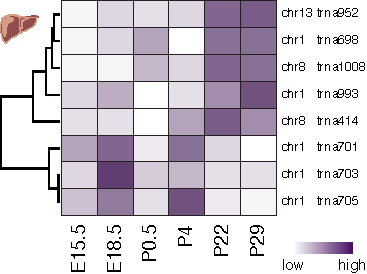
\includegraphics[height=6cm]{correlation-cag}
        \subcaption{\label{fig:compensation-a}Isoacceptor \anticodon{CAG} \trna
            gene expression levels in liver across development.\\\ }
    \end{minipage}
    \hspace{0.05\textwidth}%
    \begin{minipage}{0.4\textwidth}
        \centering
        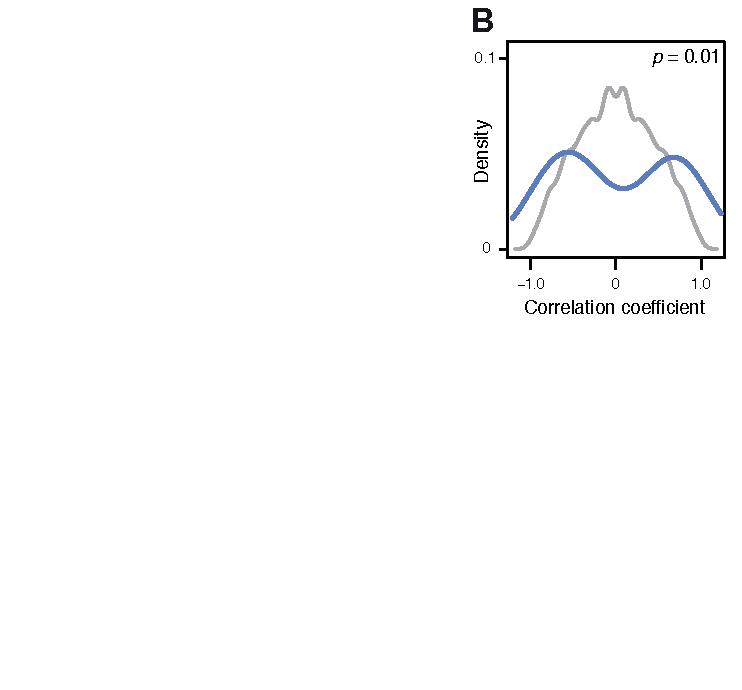
\includegraphics[height=6cm]{compensation-cag}
        \subcaption{\label{fig:compensation-b}Density curve of isoacceptor
            \anticodon{CAG} \trna gene expression correlations.}
    \end{minipage}
    \par
    \begin{minipage}{0.45\textwidth}
        \centering
        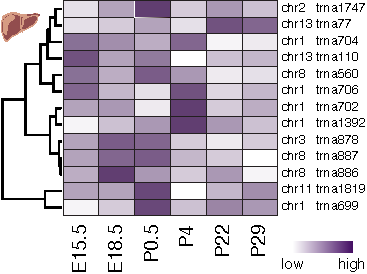
\includegraphics[height=6cm]{correlation-gcc}
        \subcaption{\label{fig:compensation-c}Isoacceptor \anticodon{GCC} \trna
            gene expression levels in liver across development.\\\ }
    \end{minipage}
    \hspace{0.05\textwidth}%
    \begin{minipage}{0.4\textwidth}
        \centering
        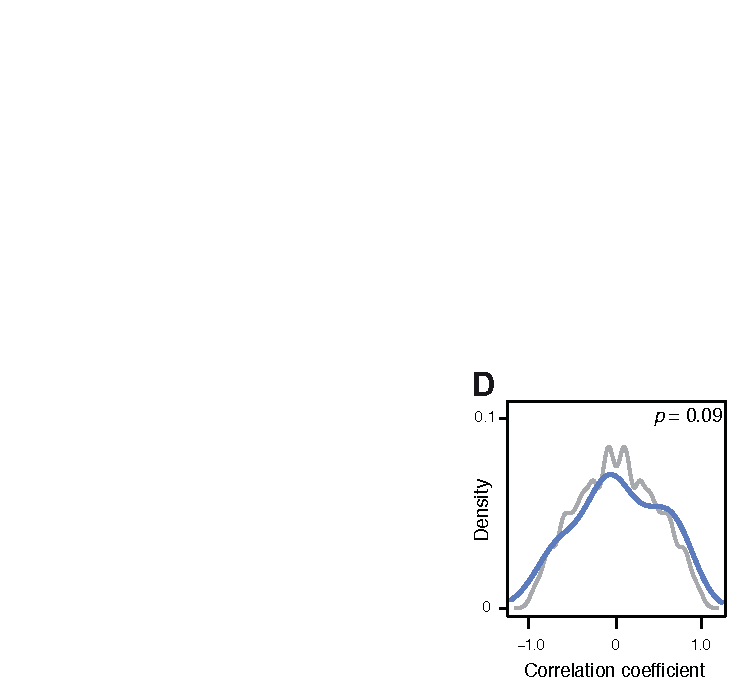
\includegraphics[height=6cm]{compensation-gcc}
        \subcaption{\label{fig:compensation-d}Density curve of isoacceptor
            \anticodon{GCC} \trna gene expression correlations.}
    \end{minipage}}
    {\trna gene expression is compensated at the anticodon isoacceptor level
    during mouse development.}
    {Panels (a) and (c) show two examples of \trna gene isoacceptor families and
    their gene expression across development (row-normalised). In panel (a) we
    can see two clusters of coordinated expression: the top \num{5} genes are
    lowly expressed at first, and start being highly expressed at P22. The
    bottom \num{3} genes show a roughly opposite trend. In panel (c), no such
    clusters are obviously present. Panels (b) and (d) show the corresponding
    pairwise gene--gene correlation coefficients, plotted as a density curve
    (blue), as well as the density curve of the background distribution.}

\begin{table}[h!]
    \centering
    \sisetup{
        table-figures-integer=1,
        table-figures-decimal=2,
        table-figures-exponent=2,
        table-sign-exponent=true,
        table-number-alignment=right
    }
    \begin{tabular}{@{}l@{}S@{}}
        \toprule
        Isoacceptor & \multicolumn{1}{r@{}}{{\(p\)-value}}\\
        \midrule
        \anticodon{GUG} & 1.01E-25 \\
\anticodon{AGC} & 2.26E-12 \\
\anticodon{GCA} & 9.17E-11 \\
\anticodon{CCA} & 1.15E-10 \\
\anticodon{CUG} & 3.60E-09 \\
\anticodon{UGG} & 3.68E-07 \\
\anticodon{AAC} & 3.68E-07 \\
\anticodon{GUA} & 5.69E-06 \\
\anticodon{CAU} & 8.53E-06 \\
\anticodon{UUC} & 2.42E-05 \\
\anticodon{UGC} & 2.56E-05 \\
\anticodon{AGA} & 6.57E-05 \\
\anticodon{CUC} & 6.81E-05 \\
\anticodon{CAC} & 2.06E-04 \\
\anticodon{GUC} & 8.76E-04 \\
\anticodon{CAG} & 1.99E-02 \\
\anticodon{GUU} & 6.01E-02 \\
\anticodon{AGU} & 1.26E-01 \\
\anticodon{GCC} & 1.33E-01 \\
\anticodon{UUU} & 3.35E-01 \\
\anticodon{GCU} & 3.45E-01 \\
\anticodon{AAU} & 3.45E-01 \\
\anticodon{GAA} & 6.50E-01 \\
\anticodon{ACG} & 8.01E-01 \\
\anticodon{UCC} & 8.01E-01 \\
\anticodon{CUU} & 8.12E-01 \\
\anticodon{AGG} & 8.44E-01 \\

        \bottomrule
    \end{tabular}

    \tabcap{compensation}{Evidence against absence of compensation.}
    {The first column contains the \trna anticodon isoacceptor families. The
    second column contains the \abbr{fdr}-adjusted \(p\)-values of \(H_0\):
    there is no effect of the order of the stages on coordinated gene expression
    of \trna genes within an isoacceptor family.}
\end{table}
